\documentclass{article}
\usepackage[utf8]{inputenc}
\usepackage{amsmath}
\usepackage{tikz}
\usetikzlibrary{positioning}
\usepackage[utf8]{inputenc}
\usepackage[english]{babel}
\newtheorem{theorem}{Theorem}
\title{ReadmeJuliaNN}
\author{Milos Vukadinovic}
\date

\begin{document}
\maketitle
\tikzset{%
  every neuron/.style={
    circle,
    draw,
    minimum size=1cm
  },
  neuron missing/.style={
    draw=none, 
    scale=4,
    text height=0.333cm,
    execute at begin node=\color{black}$\vdots$
  },
}

\begin{figure}[htp]
\centering

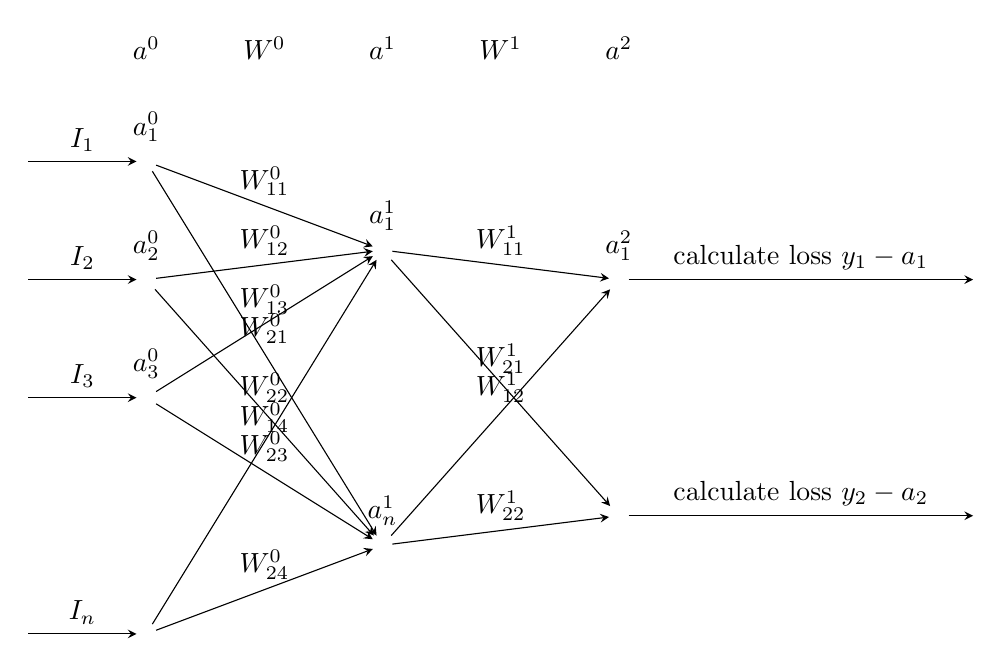
\begin{tikzpicture}[x=1.5cm, y=1.5cm, >=stealth]

\foreach \m/\l [count=\y] in {1,2,3,missing,4}
  \node [every neuron/.try, neuron \m/.try] (input-\m) at (0,2.5-\y) {};

\foreach \l [count=\y] in {1,2,3}
  \node [above] at (input-\y.north) {$a^0_\l$};
  
\foreach \m [count=\y] in {1,missing,2}
  \node [every neuron/.try, neuron \m/.try ] (hidden-\m) at (2,2-\y*1.25) {};
  
\foreach \m [count=\y] in {1,missing,2}
  \node [every neuron/.try, neuron \m/.try ] (output-\m) at (4,1.5-\y) {};

\foreach \l [count=\i] in {1,2,3,n}
  \draw [<-] (input-\i) -- ++(-1,0)
    node [above, midway] {$I_\l$};

\foreach \l [count=\i] in {1,n}
  \node [above] at (hidden-\i.north) {$a^1_\l$};

\foreach \l [count=\i] in {1,n}
  \draw [->]  (output-\i)  -- ++(3,0)
    node  [above, midway] {calculate loss $y_\i-a_\i$};
    
\foreach \l [count=\i] in {1}
  \node [above] at (output-\i.north) {$a^2_\l$};
  
\foreach \i in {1,...,4}
  \foreach \j in {1,...,2}
    \draw [->] (input-\i) -- (hidden-\j)
        node [above,midway] {$W^0_{\j\i}$};

\foreach \i in {1,...,2}
  \foreach \j in {1,...,2}
    \draw [->] (hidden-\i) -- (output-\j)
    node [above,midway] {$W^1_{\j\i}$};


\foreach \l [count=\x from 0] in {$a^0$, $a^1$, $a^2$}
  \node [align=center, above] at (\x*2,2) {\l \\ };
 \foreach \l [count=\x from 0] in {$W^0$, $W^1$}
  \node [align=center, above] at (\x*2+1,2) {\l \\ };
\end{tikzpicture}
\caption{Neural network structure and notation}
\label{neural_net}
\end{figure}
\newpage
\section{Notation}
\textit{Activation of each neuron:}
\newline
\newline
\textbf{$a_i^l$} where $l$ is the index of the layer the neuron is in and $i$ is the index of the neuron.
\newline
\newline
\textit{Weight connecting two neurons}
$w^l_{jk}$ where $l$ is the layer this weight is sending signals to (the next layer), $j$ is the index of a neuron in $l$ (to) layer and $k$ is the index of a neuron in $l-1$ (from) layer. See why we use this notation \ref{sec:indexing}
\newline
\newline
\textit{Denote notation to make things easier}
\newline
$$z_j^l = \sum_{k} w_{jk}^l a_k^{l-1}$$
Also note that 
$$a_j^l = \sigma(\sum_{k} w_{jk}^l a_k^{l-1})$$
where $\sigma$ is the sigmoid fcn
\textit{Cost function}
\newline
A cost or loss function calculates bad did our network do, higher the cost function more changes we'll need to make. It accepts the activations from the last layer $a^n$ and the correct labels $y$. In our example we will use MSE - Mean Squared Error. (We will denote last layer as $n$.
$$ C(a^n,y) = \frac{1}{2n} \sum_i (y_i - a_i^n)^2 $$
\section{Assumptions}
\begin{itemize}
    \item $C = \frac{1}{n} \sum_x C_x$
    \item Cost can be written as a fcn of the NN's output
\end{itemize}

\section{Explaining $W$ indexing}
\label{sec:indexing}
We think of $W$ as a matrix operator so that we can do matrix multiplication as follows
$$w^l a^{l-1} = a^l$$
\[
\begin{bmatrix}
$w_{11}$ & $w_{12}$ & $w_{13}$ \\
$w_{21}$ & $w_{22}$ & $w{23}$
\end{bmatrix}
\begin{bmatrix}
$a_{1}^{l-1}$\\
$a_{2}^{l-1}$ \\
$a_{3}^{l-1}$
\end{bmatrix} = 
\begin{bmatrix}
$a_{1}^l $\\
$a_{2}^l $
\end{bmatrix}
\]
\newline
Note the dimensions for the example $[2 \times 3] [3 \times 1] = [2 \times 1]$
Thus you can see why $$ w_{jk} a_{k} = a_{j}$$
\newpage
\section{Backpropagation - Calculate Gradient}
Now we will prove 3 formulas that will let us calculate the gradient for each $w$ in the network and update it. 
\newline
Let's start with calculating the partial derivative of the last (n) layer:
$$ \frac{\partial C}{\partial a_j^n} = \frac{\partial(\frac{1}{2}\sum_i (y_i - a_i^n)^2 }{\partial a_j^n} = (a_j - y_j) $$
$a_j$ is present only in one sum so the derivative is straightforward
\newline
Written in a matrix form
$$ \frac{\partial C}{\partial a^n} = (a^n - y) $$
Now, going backwards, we will calculate a partial with respect to $z^n$
$$ \frac{\partial C}{\partial z^n} = \frac{\partial C}{\partial a^n} \frac{\partial a^n}{\partial z^n} = (a^n-y) \sigma'(z^n) $$
For the simplicity we will define
$$ \delta^l = \frac{\partial C}{\partial z^l}$$
So in general we have the formula:
\begin{equation}
\delta^l = \frac{\partial C}{\partial a^l} \odot \sigma'(z^l)
\end{equation}
\newline
We have the beginning, let's build a formula to propagate the network.
We want to get $\delta^l$ in terms of $\delta^{l+1}$
$$ \frac{\partial C}{\partial z_j^l} = \frac{\partial C}{\partial z^{l+1} } \frac{\partial z^{l+1}} {\partial z^l_j} = \delta ^{l+1} \frac{\partial z^{l+1}}{\partial z^l_j}  = \delta ^{l+1}
\frac{\partial z^{l+1}}{\partial a^l_j} \frac{\partial a_j^l}{\partial z^l_j} =  \delta ^{l+1}
\frac{\partial z^{l+1}}{\partial a^l_j} \sigma'(z_j^l)$$
Now let's simplify $\frac{\partial z^{l+1}}{\partial a^l_j}$ and then we will put it back in the equation.
$$ \frac{\partial z^{l+1}}{\partial a^l_j} = 
\frac{\partial(\sum_i \sum_k w_{kj}^{l+1} a_i^{l+1})}{\partial a_j^{l+1}} = \sum_k w_{kj}^{l+1}
$$
Putting back we get 
$$\delta ^{l} = \delta ^{l+1}
\sum_k w_{kj}^{l+1} \sigma'(z_j^l)$$ 
Or in the matrix form
\begin{equation}
    \delta^l = w^{l+1} \delta^{l+1} \odot \sigma'(z^l) 
\end{equation}
This last formula is huge because it allows us to propagate back through the layers.
\newline
Finally, one left thing to do is calculate gradient for weights.
$$ \frac{\partial C}{\partial w_{jk}^l} = \frac{\partial C}{\partial z_j^l} \frac{\partial z_j^l}{\partial w_{jk}^l} = \delta_j^l a_k^{l-1}$$
We don't need to find a formula for bias because I implemented a bias trick 
In the matrix form
\begin{equation}
\frac{\partial c}{\partial w^l} = a^{l-1} \delta^l
\end{equation}
With formulas (1) (2) and (3) we are able to backpropagate!



(TODO:reference bias trick).
(TODO: add proper citations)
The whole implementation is based on the ideas from the book
Neural Network by Michael Nielsen
http://neuralnetworksanddeeplearning.com/
\end{document}
